%----------------------------------------------------------------------------------------
%	PACKAGES AND OTHER DOCUMENT CONFIGURATIONS
%----------------------------------------------------------------------------------------

\documentclass[a0,portrait]{a0poster}

\usepackage{multicol} % This is so we can have multiple columns of text side-by-side
\columnsep=100pt % This is the amount of white space between the columns in the poster
\columnseprule=3pt % This is the thickness of the black line between the columns in the poster

\usepackage[svgnames]{xcolor} % Specify colors by their 'svgnames', for a full list of all colors available see here: http://www.latextemplates.com/svgnames-colors

\usepackage{times} % Use the times font
%\usepackage{palatino} % Uncomment to use the Palatino font

\usepackage{graphicx} % Required for including images
\graphicspath{{figures/}} % Location of the graphics files
\usepackage{booktabs} % Top and bottom rules for table
\usepackage[font=large,labelfont=bf]{caption} % Required for specifying captions to tables and figures
\usepackage{amsfonts, amsmath, amsthm, amssymb} % For math fonts, symbols and environments
\usepackage{wrapfig} % Allows wrapping text around tables and figures
\usepackage{adjustbox}
\usepackage{hyperref}
\hypersetup{linkcolor=blue,citecolor=blue,filecolor=black,urlcolor=MidnightBlue} % Link colors
\usepackage{varwidth}
\newcommand\Umbruch[2][10cm]{\begin{varwidth}{#1}\centering#2\end{varwidth}}
\newcommand\Absatz[2][7cm]{\begin{varwidth}{#1}\flushleft#2\end{varwidth}}
\usepackage{tikz}
\usetikzlibrary{arrows.meta}
\tikzset{%
  >={Latex[width=2mm,length=2mm]},
  % Specifications for style of nodes:
            base/.style = {rectangle, rounded corners, draw=black,
                           minimum width=4cm, minimum height=1cm,
                           text centered, font=\sffamily},
  activityStarts/.style = {base, fill=blue!30},
       startstop/.style = {base, fill=red!30},
    activityRuns/.style = {base, fill=green!30},
         process/.style = {base, minimum width=2.5cm, fill=orange!15,
                           font=\ttfamily},
}

\begin{document}

%----------------------------------------------------------------------------------------
%	HEADER 
%----------------------------------------------------------------------------------------

% The header is divided into two boxes:
% The first is 75% wide and houses the title, subtitle, names, university/organization and contact information
% The second is 25% wide and houses a logo for your university/organization or a photo of you
% The widths of these boxes can be easily edited to accommodate your content as you see fit

\begin{minipage}[b]{1\linewidth}
\veryHuge \color{NavyBlue} \textbf{Konzept und Realisierung eines virtuellen Themenrundgangs der Fakultät Informatik zur Unterstützung bei der Studienwahl} \color{Black}\\ % Title
\Huge\textit{Handout Viculum}\\[2cm] % Subtitle
\huge \textbf{Prof. Dr. Jörg Röhrle}\\[0.5cm] % Author(s)
\huge Domenico Milazzo (TI)\\[0.3cm] % University/organization
\huge Maik Dürr (TI)\\[0.3cm] % University/organization
\huge Fabian Altenberg (WIN)\\[0.3cm] % University/organization

\end{minipage}
%

\vspace{1cm} % A bit of extra whitespace between the header and poster content

%----------------------------------------------------------------------------------------

\begin{multicols}{2} % This is how many columns your poster will be broken into, a portrait poster is generally split into 2 columns


%----------------------------------------------------------------------------------------
%	EINLEITUNG
%----------------------------------------------------------------------------------------


\section*{\huge Einleitung}

{\LARGE Viculum ist ein virtuelles Curriculum um die Modulhandbücher jeder Veranstaltungen der Hochschule Albstadt-Sigmaringen mit verschiedensten Medien und einem dynamischen Zugriff aus einer Datenbank zu visualisieren.\\}

%----------------------------------------------------------------------------------------
%	IDEEN & FEATURES
%----------------------------------------------------------------------------------------
\vspace{1cm} % A bit of extra whitespace between the header and poster content
\color{Black} % DarkSlateGray color for the rest of the content

\section*{\huge Features}

\begin{itemize}
\item {\LARGE Oracle Datenbank als Speichermedium}
\item {\LARGE Unity als Visualisierung Tool der Virtual Reality}
\item {\LARGE Dynamischen Aufbau der Szenen um Objekte}
\item {\LARGE Bilder \& Video als zusätzliche Medien}
\end{itemize}


%------------------------------------------------
\vspace{1cm} % A bit of extra whitespace between the header and poster content
\section*{\huge Datenzugriff}
\begin{center}
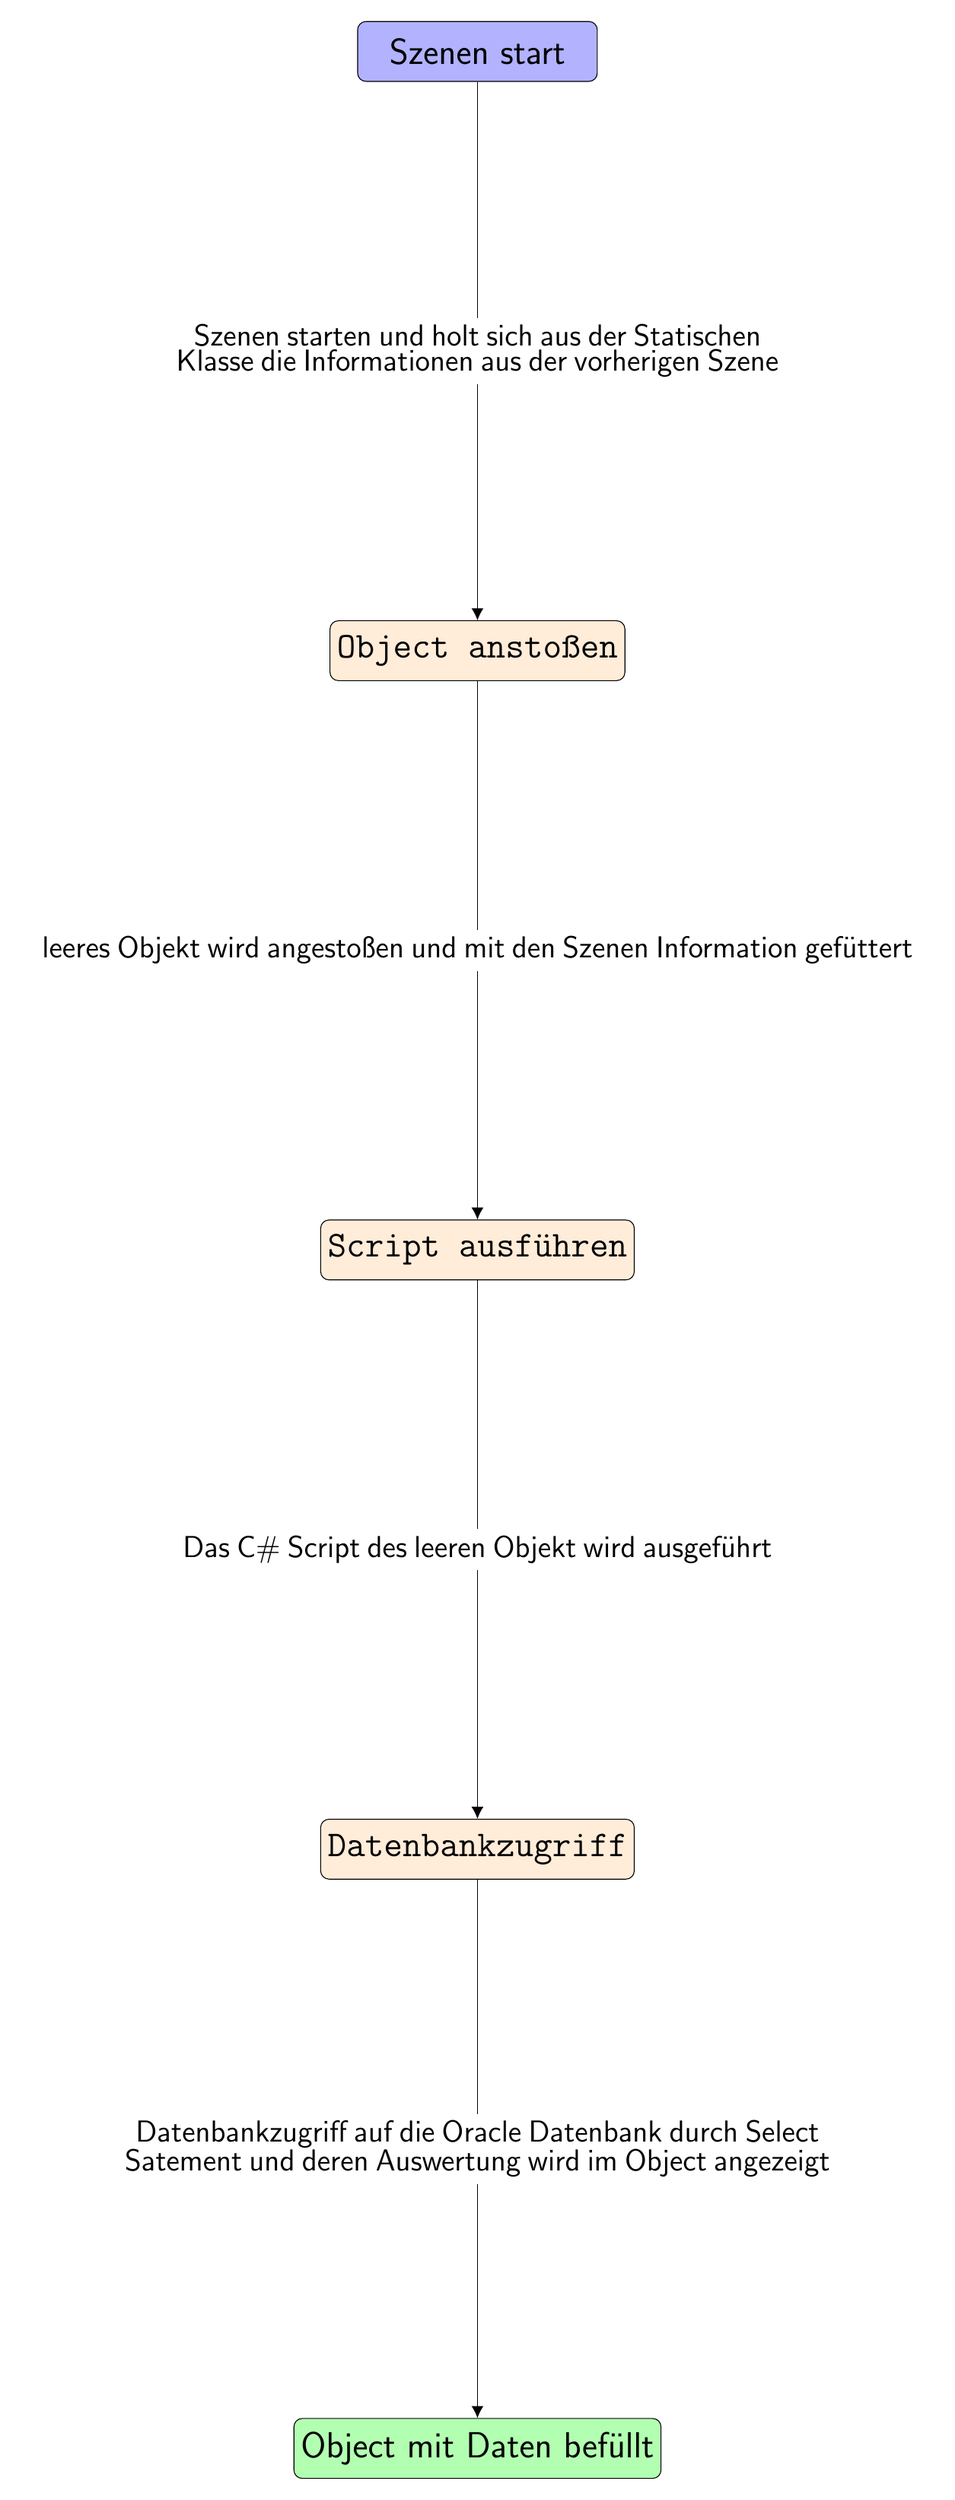
\begin{tikzpicture}[node distance=10cm,
    every node/.style={fill=white, font=\sffamily}, align=center]
  % Specification of nodes (position, etc.)
  \node (start)             [activityStarts]              	{\LARGE Szenen start};
  \node (GameObject)     [process, below of=start]  {\LARGE Object anstoßen};
  \node (Script)      [process, below of=GameObject]{\LARGE Script ausführen};
  \node (DB)     [process, below of=Script]   		{\LARGE Datenbankzugriff};
  \node (end)      [activityRuns, below of=DB]		{\LARGE Object mit Daten befüllt};   
  % Specification of lines between nodes specified above
  % with aditional nodes for description 
  \draw[->]             (start) -- node[text width=15cm]{\Large Szenen starten und holt sich aus der Statischen Klasse die Informationen aus der vorherigen Szene}(GameObject);
  \draw[->]     		(GameObject) -- node[text width=15cm]{\Large leeres Objekt wird angestoßen und mit den Szenen Information gefüttert}(Script);
  \draw[->]      		(Script) -- node[text width=15cm]{\Large Das C\# Script des leeren Objekt wird ausgeführt}(DB);
  \draw[->]     		(DB) -- node[text width=15cm]{\Large Datenbankzugriff auf die Oracle Datenbank durch Select Satement und deren Auswertung wird im Object angezeigt}(end);
  \end{tikzpicture}
\end{center}

%----------------------------------------------------------------------------------------
%	CONCLUSIONS
%----------------------------------------------------------------------------------------


\section*{\huge Aussichten}

\begin{itemize}
\item {\LARGE Pellentesque eget orci eros. Fusce ultricies, tellus et pellentesque fringilla, ante massa luctus libero, quis tristique purus urna nec nibh. Phasellus fermentum rutrum elementum. Nam quis justo lectus.}

\item {\LARGE Vestibulum sem ante, hendrerit a gravida ac, blandit quis magna.}

\item {\LARGE Donec sem metus, facilisis at condimentum eget, vehicula ut massa. Morbi consequat, diam sed convallis tincidunt, arcu nunc.}

\item {\LARGE Nunc at convallis urna. isus ante. Pellentesque condimentum dui. Etiam sagittis purus non tellus tempor volutpat. Donec et dui non massa tristique adipiscing.}
\end{itemize}

\vspace{2cm} % A bit of extra whitespace between the header and poster content


%----------------------------------------------------------------------------------------
%	Kontaktdaten 
%----------------------------------------------------------------------------------------
\color{Black}
\section*{\huge Kontaktdaten}


\vspace{1cm} % A bit of extra whitespace between the header and poster content

{\huge Domenico Milazzo}\\[1cm] % Your name
{\LARGE 
Wahlentalstraße 38\\
72461 Albstadt\\
Telefon: \texttt{0172/2441256}\\ % Your phone number
Email: \href{mailto:milazzdo@hs-albsig.de}{milazzdo@hs-albsig.de} % Your email address

}
\hrule
\vspace{2cm} % A bit of extra whitespace between the header and poster content

{\huge\flushleft Maik Dürr}\\[1cm] % Your name
{\LARGE 
Wahlentalstraße 38\\
72461 Albstadt\\
Telefon: \texttt{0172/2441256}\\ % Your phone number
Email: \href{mailto:duerrmai@hs-albsig.de}{duerrmai@hs-albsig.de} % Your email address

}
\hrule
\vspace{2cm}

{\huge\flushleft Fabian Altenberg}\\[1cm] % Your name
{\LARGE 
Wahlentalstraße 38\\
72461 Albstadt\\
Telefon: \texttt{0172/2441256}\\ % Your phone number
Email: \href{mailto:altenbfa@hs-albsig.de}{altenbfa@hs-albsig.de} % Your email address

}
\hrule
\vspace{2cm}



\includegraphics[width=0.3\textwidth]{hsas_logo.png}
\end{multicols}
\end{document}